\documentclass[11pt]{article}
\usepackage{fullpage}
\usepackage{graphicx}

\newcommand {\doublespace} {\addtolength{\baselineskip}{.5\baselineskip}}
\newcommand {\singlespace} {\addtolength{\baselineskip}{-.333\baselineskip}}

\newtheorem{lemma}{Lemma}[section]
\newtheorem{theorem}{Theorem}[section]
\newtheorem{corollary}{Corollary}[section]
\newtheorem{definition}{Definition}[section]
\newtheorem{conjecture}{Conjecture}[section]

\def\Proof{\par\noindent{\sl Proof\/}:\enspace}
\def\blackslug{\hbox{\hskip 1pt \vrule width 4pt height 8pt depth 1.5pt
  \hskip 1pt}}
\def\QED{\quad\blackslug\lower 8.5pt\null}

\begin{document}

\title{Fractal Dimension Calculation}
\author{Stephen R. Tate\\Department of Computer Science\\UNC Greensboro}
\date{December 28, 2017}

\maketitle

The purpose of this document is to describe how fractal dimensions are
calculated in the JavaScript ``\texttt{fracexpl.js}'' fractal
explorer. A fractal is defined by a seed shape made up of individual
segments, where each segment represents either a scaled version of the
fractal or a simple line segment. For example, the seed shape on the
left below defines the Koch curve (rendered on the right), where each
segment is a replicating segment of length 5, and the length of the
baseline (the dashed line) is 16.

\begin{center}
\includegraphics[scale=0.9]{kochexample.pdf}
\end{center}
We denote the size (either
length or area) of a shape with baseline length $b$ as $S(b)$. For a
shape with dimension $d$, the function should satisfy
\[ S(b)= k\cdot b^d \]
for some constant $k$.
For example, when the shape is a line segment that is twice the length
of the baseline, then $S(b)=2b$, so the dimension is 1. When the shape
is a rectangle that is $b$ units on one side and $3b$ on the other
side, then $S(b)=3b^2$ so the dimension is 2.

For regular fractals, such as the Koch curve, every segment of the
seed shape is replicated and of the same length, and we can solve for
$d$ analytically. In the Koch seed above, each of the 4 replicating
segments has length $\frac{5}{16} b$, so
$4 S(\frac{5}{16} b) = S(b)$ for all $b$.  We plug into our
general form for $S(b)$ to get
\[ 4 k \left(\frac{5}{16} b\right)^d = k\cdot b^d
\iff \left(\frac{16}{5}\right)^d = 4 \iff d = \frac{\log 4}{\log 3.2} = 1.191844...
\]
Therefore, this Koch curve has dimension approximately 1.19.

Unfortunately, when you get beyond regular seed shapes and when you
put in non-replicating line segments, analytic solutions are
impossible. For the general case, consider a seed shape
in which there are $n$ replicating segments, with lengths
$c_1b,c_2b,\cdots,c_nb$, and
$m$ fixed (non-replicating) segments with lengths
$f_1b,f_2b,\cdots,f_mb$. The size of the fractal then satisfies
\begin{equation}
\label{eq:general}
S(b) = \sum_{i=1}^k S(c_i b) + \sum_{i=1}^m f_i b .
\end{equation}
Consider two cases: when $m=0$ (i.e., there are no non-replicating
segments), and when $m>0$.

\par\vspace*{1.5ex}\noindent
\textbf{Case 1: $m=0$.}
In this case, the second sum in~(\ref{eq:general}) is empty, so
\[ \sum_{i=1}^n S(c_i b) = S(b)
   \iff k\cdot b^d = \sum_{i=1}^n k\cdot (c_i b)^d 
   \iff \sum_{i=1}^n c_i^d = 1
\]
For a given seed shape (i.e., for given $c_i$ values), the
\texttt{fracexpl.js} code solves this equation using 
bisection.

\par\vspace*{1.5ex}\noindent
\textbf{Case 2: $m>0$.} In this case we must consider the full formula
in~(\ref{eq:general}), so we need
\[ \sum_{i=1}^k S(c_i b) + \sum_{i=1}^m f_i b = S(b)
\iff
\sum_{i=1}^n k\cdot (c_i b)^d + \sum_{i=1}^m f_i b = k\cdot b^d
\iff
b^d \sum_{i=1}^n c_i^d + \frac{b}{k} \sum_{i=1}^m f_i = b^d
. \]
This equation must hold for all values of $b$ (since dimension is
scale-invariant), and it is not hard to
see that if the sum of the $f_i$'s is non-zero this can only hold when
$d=1$. Fixing $d=1$, we get
\[
\sum_{i=1}^n c_i + \frac{1}{k} \sum_{i=1}^m f_i = 1
\iff
k = \frac{\sum_{i=1}^m f_i}{1-\sum_{i=1}^n c_i} .
\]
We can solve for a positive $k$ if and only if $\sum_{i=1}^n c_i < 1$,
so the \texttt{fracexpl.js} code tests for this special case and
returns dimension 1 if this holds. If there are non-replicating
segments and this does \emph{not} hold, then there is no way find a
scale-invariant dimension, and so the code indicates that there is
unknown dimension in this case.
\end{document}
